\subsection{Current Implementation Overview}\label{subsec:current-implementation2}
We performed multiple experiments to assess the effectiveness of our implementation by various different hyperparameters.
All the detailed results from these experiments are presented in
Appendix~\ref{sec:detailed-experiment-results} (see Table~\ref{tab:detailed-results}).
This table offers an overview of our findings and supports the analyses discussed in the following sections.


\subsection{Visualizations}\label{subsec:best-accuracy-viz2}
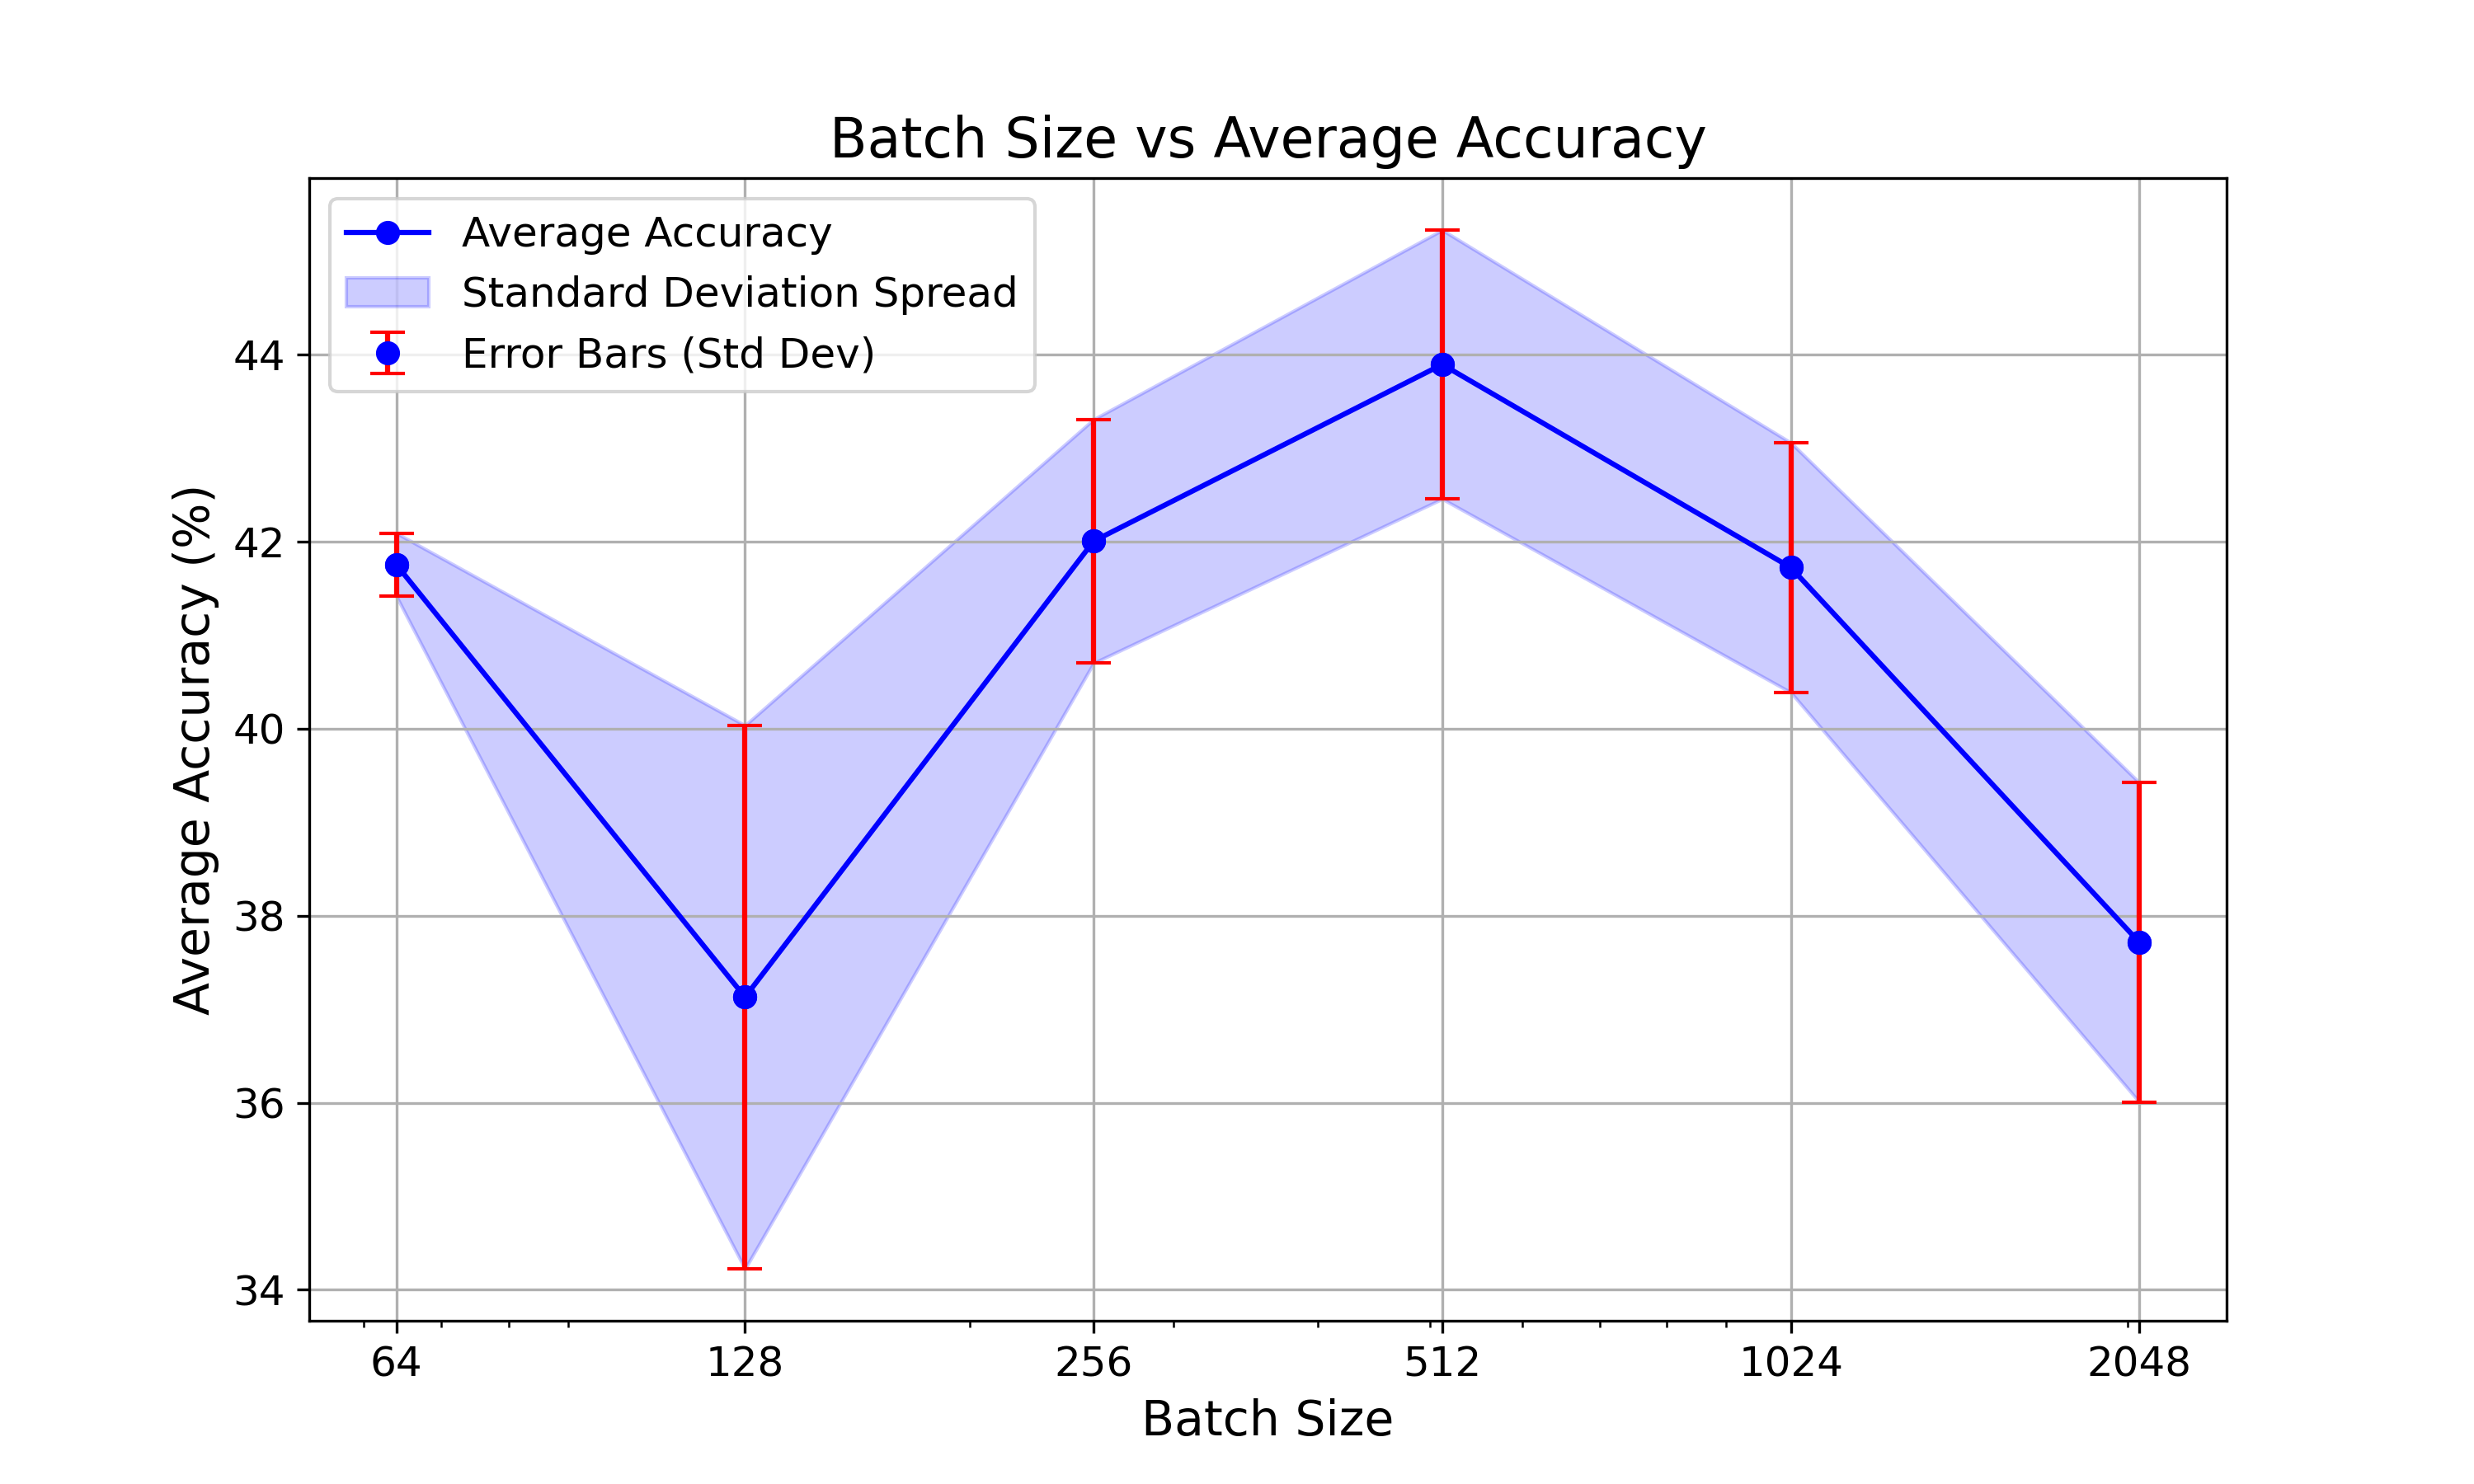
\includegraphics[width=0.7\textwidth]{batch_size_vs_accuracy.png}
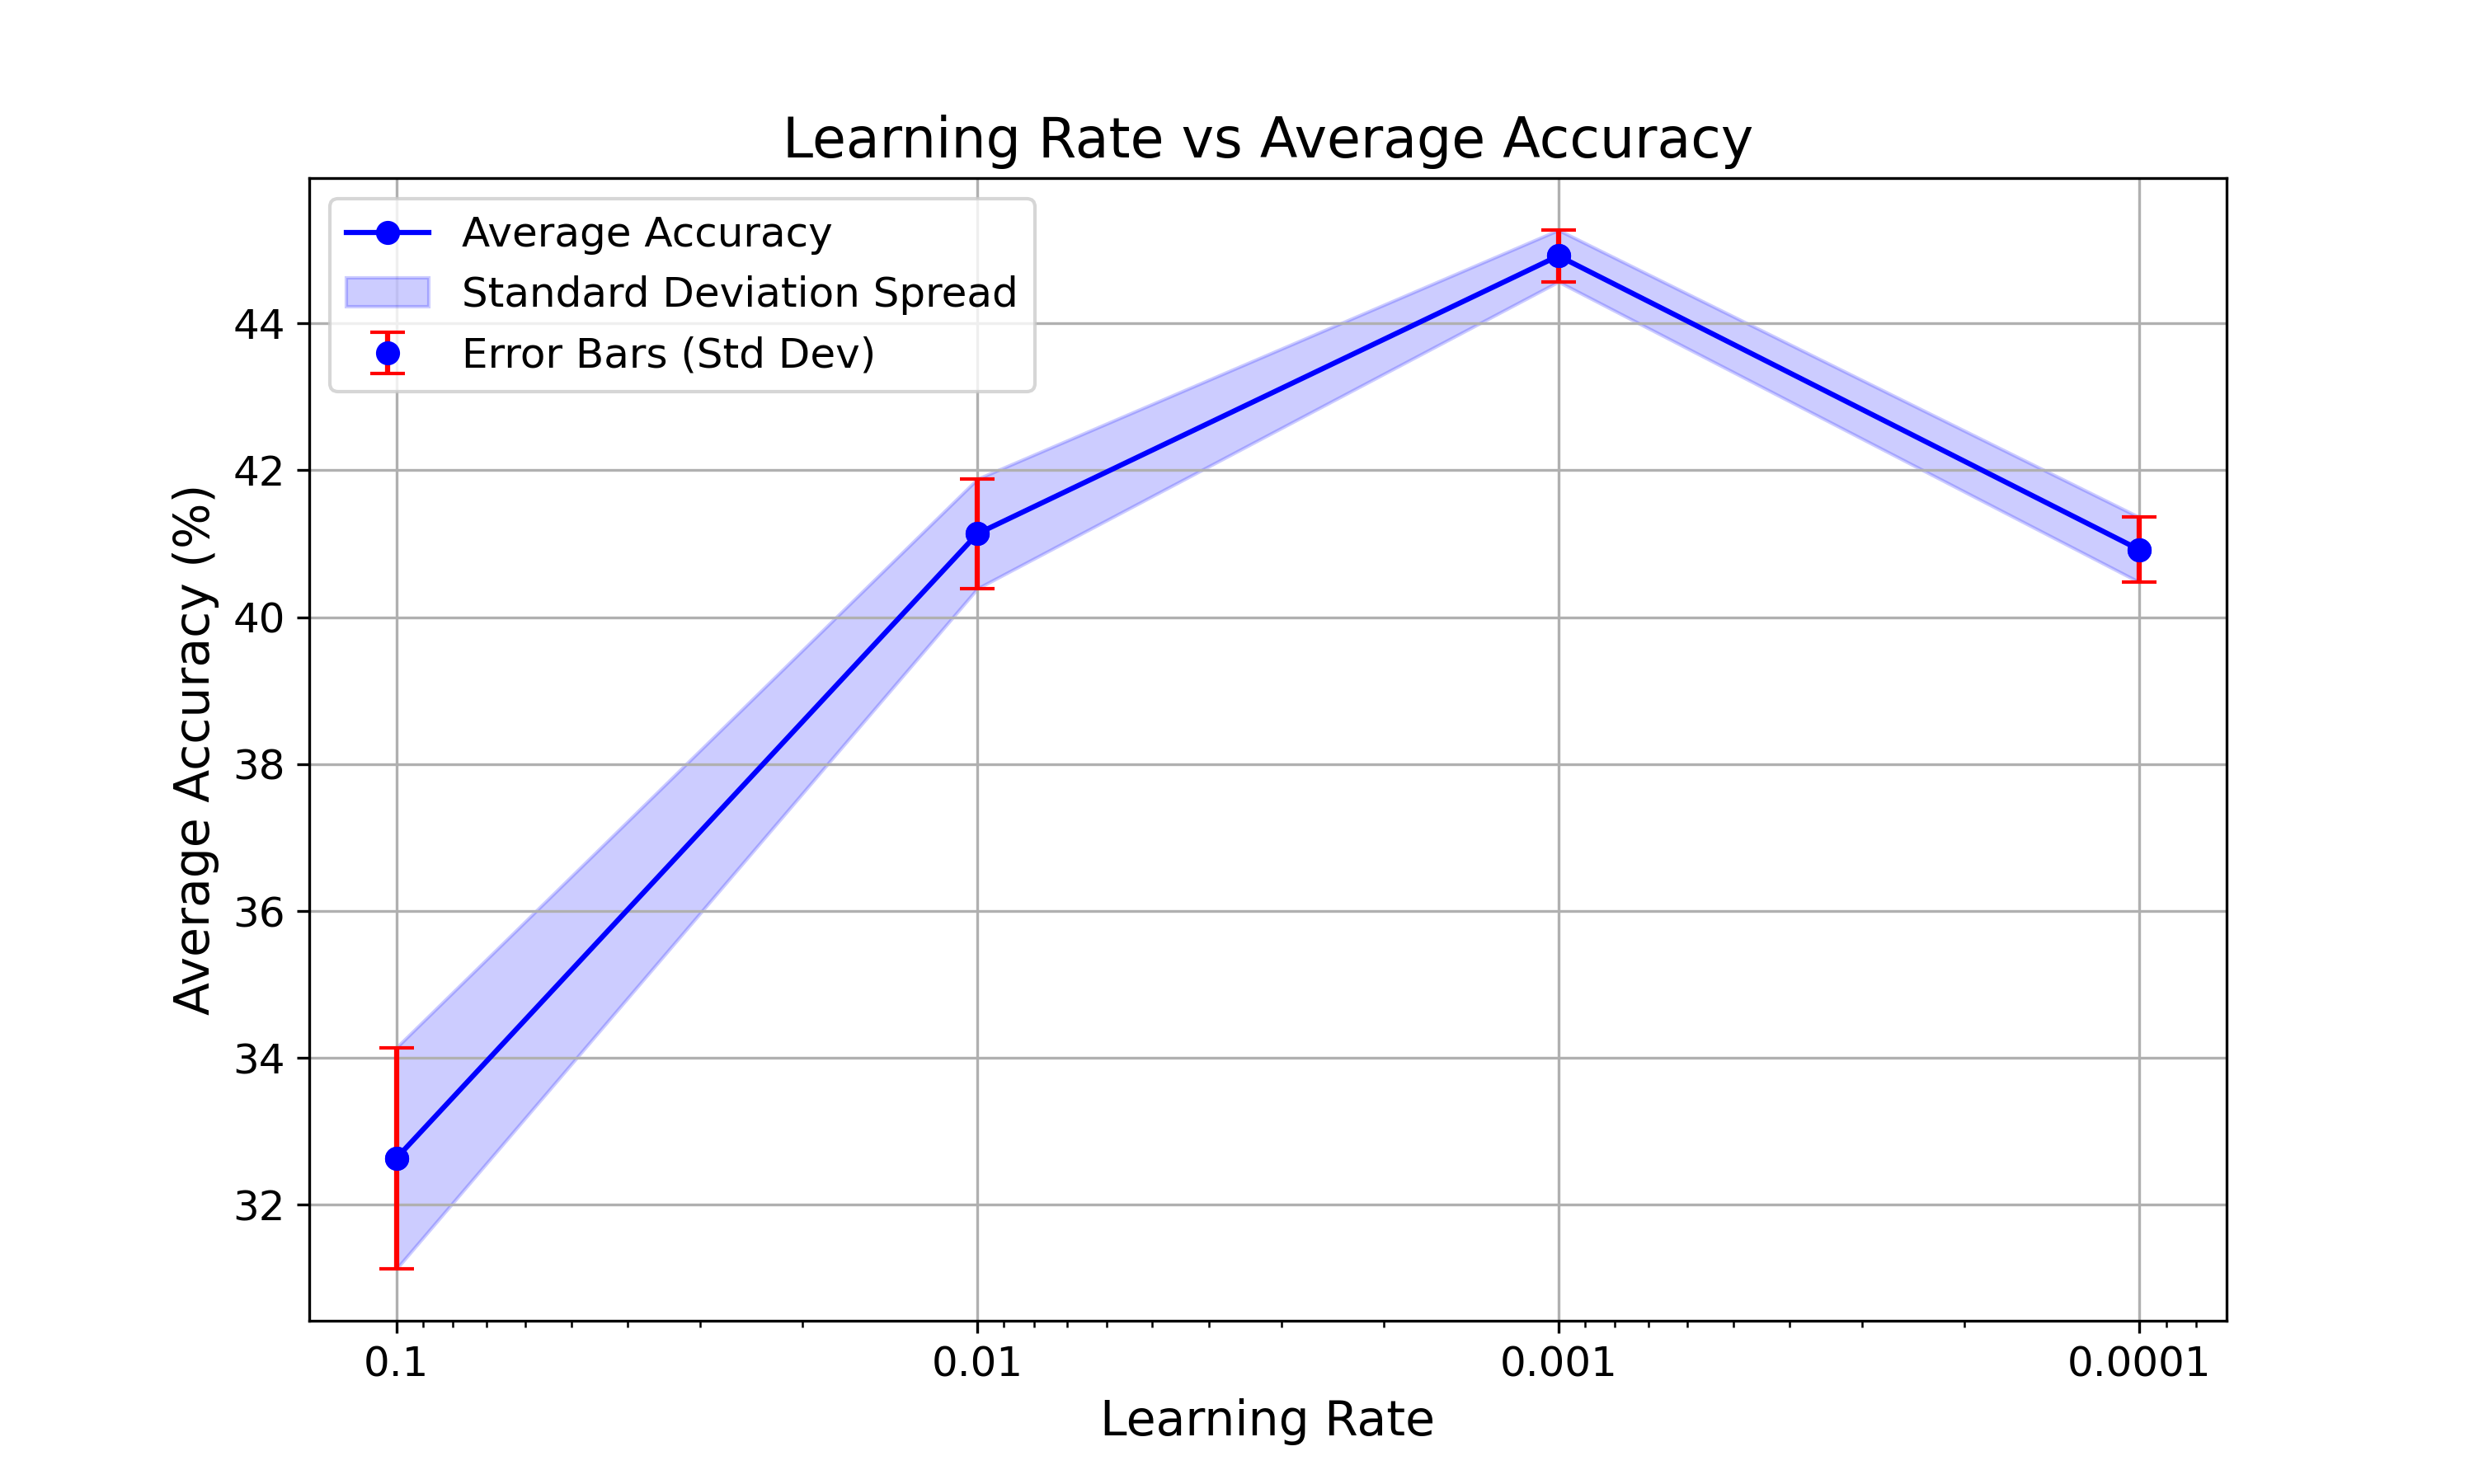
\includegraphics[width=0.7\textwidth]{learning_rate_vs_accuracy.png}
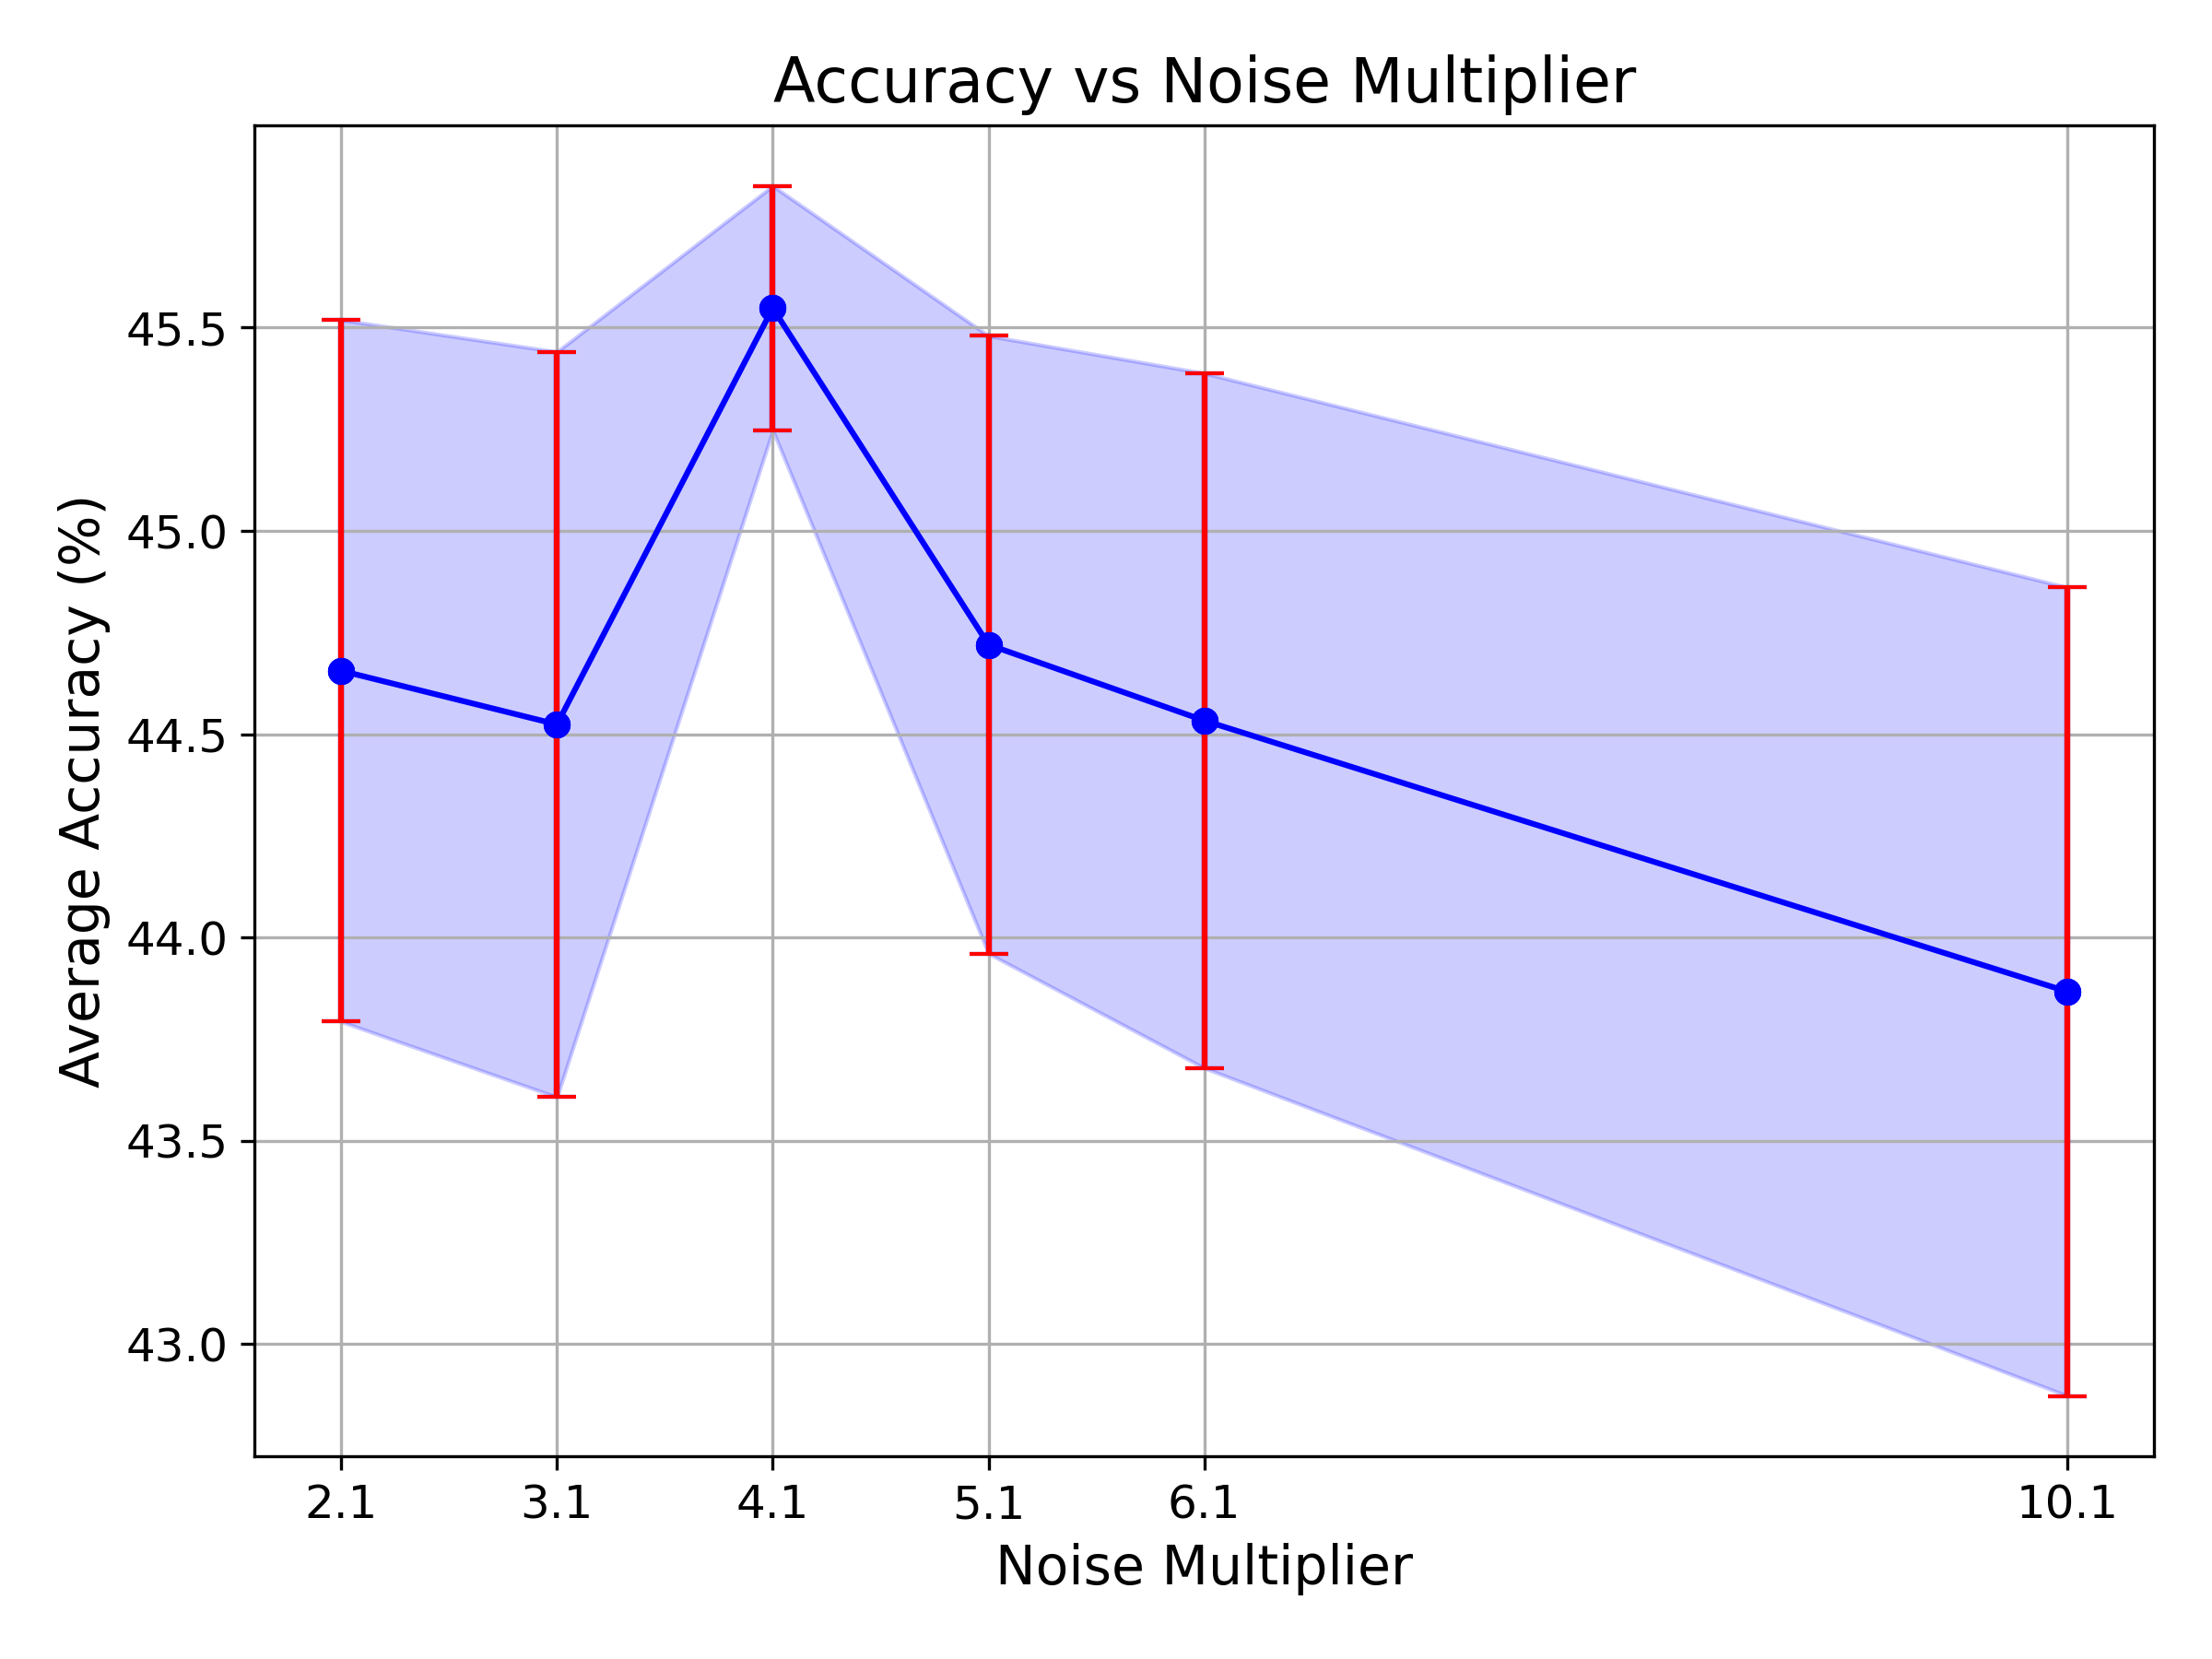
\includegraphics[width=0.7\textwidth]{Accuracy vs Noise Multiplier.png}

\subsection{Best Observed Accuracy and Components/Hyperparameters}\label{subsec:best-accuracy2}
The biggest change from the BA report \#1 was the privatization of the Lion Optimizer. To privatize, we made the gradients used in the algorithm "noisy" by introducing clipping
at the per example gradient level and then adding noise for the batch. The above results indicate the first round of testing completed with the new DP-Lion Optimizer.

We began our testing with a grid-search of possible hyperparameter combinations for batch size, learning rate, and noise multiplier. The main takeaways were that batch size,
when changed indepedently, appears to be optimal around 512 batch size. For Learning rate, it appeared that a learning rate of .001 showed the highest accuracy over a set of 5
runs. Finally, for noise multiplier, we found that raising the multiplier to 4.1 from 1.1 might provide some improvements in accuracy. We also found there to be marginal differences
between higher and lower noise multipliers when using large batch sizes.

In this suite of testing, our highest accuracy was roughly 46\%. We then turned to the original non-private Lion paper for some guidance on how they adjusted hyperparameters. They recommend 
large batch sizes and relatively small learning rates (relative to DP-Adam, DP-SGD, DP-RMSprop). They also recommend a $Beta_{1}$ value of 0.95 and a $Beta_{2}$ value of 0.98. We tested
these beta values also with increasing the epochs from 30 to 200 and achieved a peak accuracy of 54.43\%. This is the highest private accuracy we have been able to generate in our testing
yet. 

In our early testing, it seems that non-private Lion and Private Lion might prefer the same types of hyperparameters, namely large batch sizes, small learning rates, $Beta_{1}$ value of 0.95,
and a $Beta_{2}$ value of 0.98.

\begin{itemize}
    \item \textbf{Learning Rate:} We varied learning rate from 0.1 to 0.0001. The middle learning rate (0.001) yielded the highest accuracy of 45\%.
    \item \textbf{Batch Size:} We varied batch size from 64 to 2048. A batch size of 512 yielded the highest accuracy of 44\% among its peers.
    \item \textbf{Noise Multiplier:} Along with Epsilon changes, our highest accuracy, 54.43\%, also coincided with an increase in noise multiplier (10.1).
\end{itemize}

\subsection{Failed Approaches}\label{subsec:failed-approaches2}
It seems that using smaller batch sizes is not optimal for accuracy of Lion. We also notice that large learning rates like those used in DP-SGD degrade accuracy dramatically. Lastly, 
we found that $Beta_{1}$ value of 0.9 and a $Beta_{2}$ value of 0.999, which are the commonly used values for Adam, are not optimal for DP-Lion.

\subsection{Implementation Challenges}\label{subsec:implementation-challenges2}
We needed to find an implementation of Lion to be used in our model. We used the following non-private Lion implementation from the google automl repository: 
\url{https://github.com/google/automl/blob/master/lion/lion_pytorch.py}. 

From there, we needed to then pass the optimizer through the opacus make private function to return the noisy gradients optimization.
As we're looking to improve the accuracy of our models, we're needing to increase the batch size and the epochs the model runs for. This is causing us to hit a computing
limit. Some of our runs take upwards of 3600 seconds (roughly 1 hour) and can use considerable memory as well. This isn't a persistent issue, but sometimes the runs will hit memory
allocation or OOM issues on CUDA.
